\documentclass[11pt]{article}
\usepackage[margin=1in]{geometry}
\usepackage{amsmath,amssymb,amsthm}
\usepackage{booktabs,graphicx,caption}
\usepackage[hidelinks]{hyperref}
\usepackage{natbib}
\newtheorem{proposition}{Proposition}
\newcommand{\e}{\varepsilon}
\setlength{\parskip}{4pt}

\title{AI Capital versus Regular Capital:\\
Real Interest Rates and Wages after Jumps, Faster Growth, and Anticipated Innovation}
\author{Research note (draft)}
\date{October 2026}

\begin{document}
\maketitle

\begin{abstract}
\noindent This note compares the dynamics of the real interest rate and the real wage
after technical progress in AI capital and after progress in regular capital. Regular
capital and labor form a Cobb-Douglas bundle, and AI capital is a substitute for that
bundle. Progress is either disembodied (in the production function) or embodied (a
falling price of new capital in the accumulation equation). Three experiments are
considered: (1) a surprise permanent jump in technology; (2) a surprise permanent
increase in its growth rate; and (3) an S-curve innovation centered on year 10 and
known at year 0. Each experiment is solved under standard linear capital accumulation
and under the moderate adjustment costs of \citet{kiley2004}. Balanced growth paths
are in closed form. For the same long-run output gain, AI progress raises the wage by
$1/[1+(1-a)(\e-1)]$ of the output gain (74 percent here), while regular-capital progress
raises it one-for-one. Embodied progress delays wage gains. With linear accumulation it
initially \emph{lowers} the real interest rate when it is ongoing or anticipated,
because firms wait for cheaper capital. Adjustment costs largely remove that effect.
Permanently faster AI progress has no balanced growth path when AI is a substitute.
\end{abstract}

\section{Model}

Notation follows \citet{kiley2000}. Production nests a Cobb-Douglas bundle of regular
capital and labor inside a CES aggregate with AI capital:
\begin{equation}
X=(\Gamma_KK)^a(ZN)^{1-a},\qquad
Y=\Big[\omega^{1/\e}X^{\frac{\e-1}{\e}}+(1-\omega)^{1/\e}(\Gamma_AA)^{\frac{\e-1}{\e}}\Big]^{\frac{\e}{\e-1}},
\qquad \e=1.5 .
\end{equation}
AI substitutes for the bundle, and therefore for both labor and regular capital. Capital $j\in\{K,A\}$ is measured
in efficiency units, and a new unit costs $P_j$ in output:
\begin{equation}
K_j'=(1-d_j)K_j+I_j/P_j .
\end{equation}
\emph{Disembodied} progress raises $\Gamma_j$, and with it the productivity of the installed stock.
\emph{Embodied} progress lowers $P_j$, which makes new capital cheaper but leaves existing units unchanged.
Two accumulation technologies are compared:
\begin{itemize}
\item \emph{Linear}: no adjustment costs.
\item \emph{Adjustment costs}: $P_j\,\tfrac{c_j}{2}(i_j-x_j)^2K_j$, with $i_j=I_j/(P_jK_j)$. The
cost vanishes at the balanced-growth investment rate $x_j$, and $c_j=1/x_j$, so that the
elasticity of $i_j$ with respect to $Q_j/P_j$ is one (the paper's ``moderate'' case).
\end{itemize}
Utility is logarithmic and hours are fixed. Calibration: $a=0.282$, $d_K=0.066$,
$d_A=0.20$, trend growth $g_Z=1.5$ percent, initial $r=7.5$ percent and an initial AI
income share of 3 percent. Because $\e>1$, the AI share rises as AI becomes cheaper.

\begin{proposition}[Balanced growth path]\label{prop:bgp}
Let $\Gamma_j$ grow at $\gamma_{\Gamma j}$ and $P_j$ fall at $\gamma_{qj}$, and write
$G_j=(1+\gamma_{\Gamma j})(1+\gamma_{qj})$. A balanced growth path exists if $\e=1$, or if
$\e\neq1$ and $G_A=1$. Output grows at
\begin{gather*}
\ln(1+g)=\ln(1+g_Z)+\frac{a\omega\ln G_K+(1-\omega)\ln G_A}{(1-a)\,\omega}\quad(\e=1),\\
\ln(1+g)=\ln(1+g_Z)+\frac{a}{1-a}\ln G_K\quad(\e\neq1).
\end{gather*}
With $1+r=(1+g)/B$, user costs $u_j=(1+r)(1+\gamma_{qj})-(1-d_j)$ and effective costs
$\lambda_j=P_ju_j/\Gamma_j$:
\begin{gather*}
s_A=(1-\omega)\lambda_A^{1-\e},\qquad \text{labor share}=(1-a)(1-s_A),\qquad
P_X^{1-\e}=\frac{1-s_A}{\omega},\\
\ln\frac WZ=\frac{1}{1-a}\ln P_X-\frac{a}{1-a}\ln\lambda_K+\text{const},\qquad
\ln\frac YZ=\ln\frac WZ-\ln(1-s_A)+\text{const}.
\end{gather*}
Adjustment costs are zero on the path, $Q_j=P_j$, and $P_KK/Y=a(1-s_A)/u_K$, $P_AA/Y=s_A/u_A$.
\end{proposition}

The embodied user cost includes an obsolescence term: $u_j\approx r+d_j+\gamma_{qj}$.

\begin{proposition}[Level shifts with the same long-run output gain $\gamma_Y$]\label{prop:level}
Disembodied and embodied progress have the same long-run effects when
$\ln\Gamma_j=-\ln P_j$. The long-run interest rate is unchanged.
\begin{enumerate}
\item \emph{Regular capital}: the AI share and labor share are unchanged, so
$\Delta\ln W=\gamma_Y$. The required shock is $\ln(\Gamma_K/P_K)=\frac{1-a}{a}\gamma_Y$.
\item \emph{AI capital}: only $s_A$ moves, and
\begin{equation*}
\Delta\ln W=\frac{\gamma_Y}{1+(1-a)(\e-1)},\qquad
\Delta\ln(\text{labor share})=\Delta\ln(1-s_A)=-\frac{(1-a)(\e-1)}{1+(1-a)(\e-1)}\,\gamma_Y .
\end{equation*}
\end{enumerate}
\end{proposition}
\emph{Proof.} From Proposition~\ref{prop:bgp}, $\ln(Y/Z)=\frac{1}{(1-a)(1-\e)}\ln(1-s_A)-\ln(1-s_A)-\frac{a}{1-a}\ln\lambda_K+$const.
Regular-capital progress moves only $\lambda_K$. AI progress moves only $s_A$, and
$\ln W=\ln Y+\ln(1-s_A)$. \qed

With $\gamma_Y=10$ percent, regular-capital progress raises the wage 10 percent and AI
progress raises it 7.4 percent. The AI share rises from 3.0 to 5.5 percent, and the labor
share falls from 69.6 to 67.8 percent. Because AI is small, the same output gain requires
$\Gamma_A/P_A$ to rise 3.4-fold, against a 29 percent rise in $\Gamma_K/P_K$.

\begin{proposition}[Faster growth]\label{prop:growth}
\emph{Regular capital}: a permanent increase in $\gamma_{\Gamma K}$ or $\gamma_{qK}$ moves the
economy to a new balanced growth path with $\Delta\ln(1+g)=\frac{a}{1-a}\ln G_K$ and
$\Delta\ln(1+r)=\Delta\ln(1+g)$, for any $\e$. The wage grows at the new rate $g$, and its
level relative to $Z$ falls because $\lambda_K$ rises. The fall is larger for embodied
progress, through the obsolescence term in $u_K$.
\emph{AI capital with $\e>1$}: there is no balanced growth path. $\lambda_A\to0$, the AI
share $\to1$, the labor share $\to0$, and growth and the interest rate rise without
bound. This is the explosive limit derived in the companion note.
\emph{AI capital with $\e=1$}: there is a balanced growth path with
$\Delta\ln(1+g)=\frac{1-\omega}{(1-a)\omega}\ln G_A$. Delivering the same growth increase as
regular-capital progress then requires AI progress about $(1-a)\omega/(1-\omega)\approx23$
times as fast as the increase in output growth.
\end{proposition}

Two equivalences organize the results. With a Cobb-Douglas bundle, disembodied
regular-capital progress is the same as labor-augmenting progress. With $\e=1$,
disembodied progress in either capital is the same as Hicks-neutral TFP growth. Its
paths are therefore identical whichever capital it attaches to. In both cases only
\emph{embodied} progress distinguishes one kind of capital from another.

\section{Experiments}

Every experiment is announced, or occurs, at $t=0$ with the economy on its initial
balanced growth path. Each is solved as a nonlinear perfect-foresight problem
(Newton's method, 250 years, residuals below $10^{-10}$). Wages are log deviations from
the pre-shock path ($W/Z$ on the initial trend). The labor share is relative to gross
output.

\subsection*{Case 1: surprise permanent jumps}

\begin{figure}[h]\centering
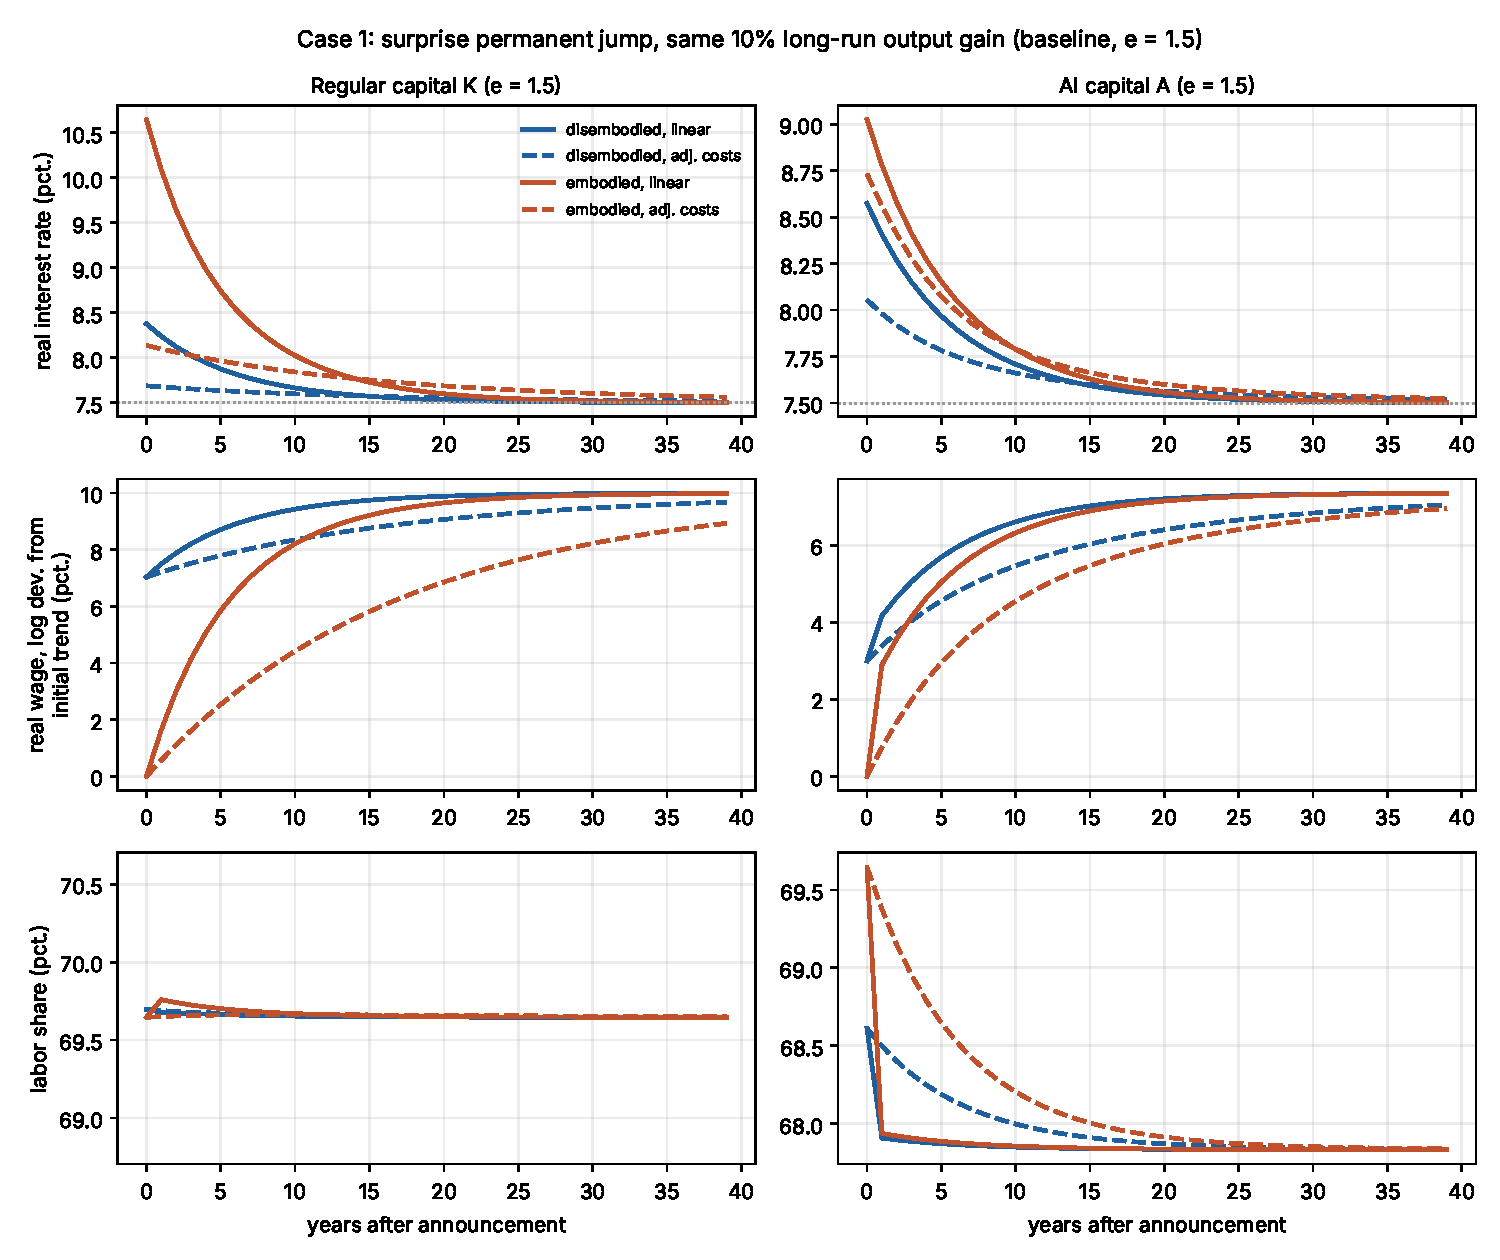
\includegraphics[width=\textwidth]{figures/fig_g_case1.pdf}
\caption{Case 1. Solid: linear accumulation. Dashed: adjustment costs.}\label{fig:c1}
\end{figure}

\begin{table}[h]\centering\scriptsize
\caption{Case 1: surprise permanent jump, same 10\% long-run output gain. The shock is in log points; $r_1$ is the rate between years 0 and 1.}\label{tab:c1}
\begin{tabular}{llccccccc}\toprule
 & & shock & $r_1$ & peak $r$ & year & $\ln W$, $t{=}10$ & $\ln W$, long run & labor share\\
 & & & (pct.) & (pct.) & & (pct.) & (pct.) & long run (pct.)\\\midrule
$K$ disemb. & linear & 0.255 & 8.38 & 8.38 & 0 & 9.4 & 10.0 & 69.6\\
$K$ disemb. & adj. costs & 0.255 & 7.69 & 7.69 & 0 & 8.4 & 10.0 & 69.6\\
$K$ emb. & linear & 0.255 & 10.64 & 10.64 & 0 & 8.2 & 10.0 & 69.6\\
$K$ emb. & adj. costs & 0.255 & 8.14 & 8.14 & 0 & 4.4 & 10.0 & 69.6\\
\midrule
AI disemb. & linear & 1.223 & 8.57 & 8.57 & 0 & 6.6 & 7.4 & 67.8\\
AI disemb. & adj. costs & 1.223 & 8.05 & 8.05 & 0 & 5.5 & 7.4 & 67.8\\
AI emb. & linear & 1.223 & 9.03 & 9.03 & 0 & 6.3 & 7.4 & 67.8\\
AI emb. & adj. costs & 1.223 & 8.73 & 8.73 & 0 & 4.5 & 7.4 & 67.8\\
\bottomrule\end{tabular}

\end{table}

\begin{enumerate}
\item \emph{Interest rates jump on impact and decay.} Embodied progress raises $r$ more than
disembodied progress, because it requires an investment boom before any output gain.
Under linear accumulation, a jump in regular-capital technology raises $r_1$ to 10.6
percent (embodied) or 8.4 percent (disembodied). For AI the figures are 9.0 and 8.6
percent. Adjustment costs damp the regular-capital response (8.1 and 7.7 percent) more
than the AI response (8.7 and 8.05 percent), because AI's adjustment cost per unit of
investment is smaller.
\item \emph{Wages.} Disembodied progress raises wages on impact, by 7.0 percent for regular
capital and 3.0 percent for AI. Embodied progress raises them only as new capital is
installed. With adjustment costs, after ten years wages are still 5.6 percentage points
short of their long-run gain for regular capital, and 2.9 points short for AI.
\item \emph{Labor share.} It is unchanged for regular capital. For AI it falls by 1.8
points, at once under disembodied progress and over 10--20 years under embodied
progress with adjustment costs.
\end{enumerate}

\subsection*{Case 2: faster growth}

Each shock raises long-run output growth by 0.5 percentage points, from 1.5 to 2.0
percent. AI growth needs $\e=1$ (Proposition~\ref{prop:growth}), so the figure and
table use the $\e=1$ variant for both capital stocks. Regular-capital results in the
$\e=1.5$ baseline are nearly identical; for example, $r_1$ under embodied progress with linear accumulation is 6.50 vs 6.48
percent.

\begin{table}[h]\centering\scriptsize
\caption{Balanced growth paths (Proposition~\ref{prop:bgp}). $\gamma$ is the annual rate of technical progress; $W/Z$ is relative to the initial path at the same date-0 technology levels. Rates in percent.}\label{tab:bgp}
\begin{tabular}{llccccccc}\toprule
 & & $\gamma$ & $g$ & $r$ & $u_K$ & $u_A$ & $W/Z$ & labor share\\\midrule
$\e=1.5$ & Initial & 0.00 & 1.50 & 7.50 & 14.10 & 27.50 & 1.000 & 69.6\\
 & $K$ disembodied, $\gamma$ & 1.26 & 2.00 & 8.03 & 14.63 & 28.03 & 0.985 & 69.7\\
 & $K$ embodied, $\gamma$ & 1.26 & 2.00 & 8.03 & 15.99 & 28.03 & 0.951 & 69.7\\
\midrule
$\e=1$ & Initial & 0.00 & 1.50 & 7.50 & 14.10 & 27.50 & 1.000 & 69.6\\
 & $K$ disembodied & 1.26 & 2.00 & 8.03 & 14.63 & 28.03 & 0.985 & 69.6\\
 & $K$ embodied & 1.26 & 2.00 & 8.03 & 15.99 & 28.03 & 0.951 & 69.6\\
 & AI disembodied & 12.08 & 2.00 & 8.03 & 14.63 & 28.03 & 0.985 & 69.6\\
 & AI embodied & 12.08 & 2.00 & 8.03 & 14.63 & 41.08 & 0.969 & 69.6\\
\bottomrule\end{tabular}

\end{table}

\begin{figure}[h]\centering
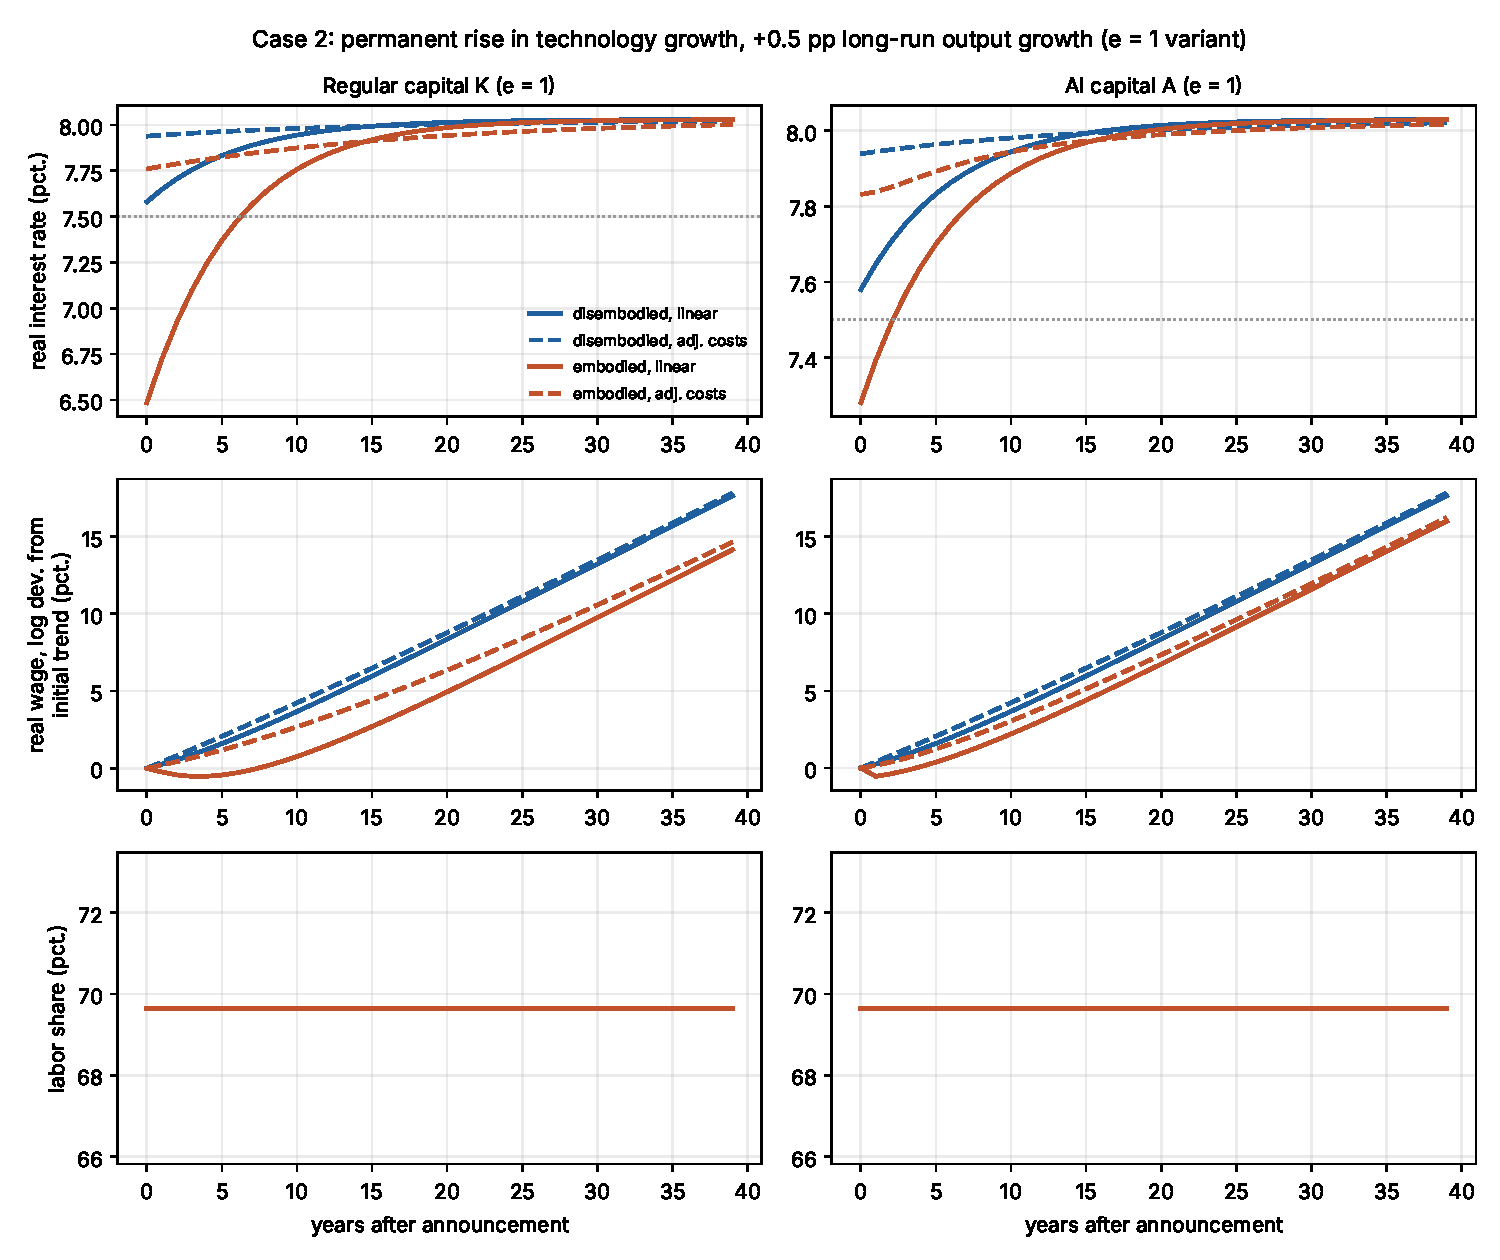
\includegraphics[width=\textwidth]{figures/fig_g_case2.pdf}
\caption{Case 2 ($\e=1$). The labor share is constant by construction when $\e=1$.}\label{fig:c2}
\end{figure}

\begin{table}[h]\centering\scriptsize
\caption{Case 2: permanent increase in the growth of technology from $t=0$ ($\e=1$).}\label{tab:c2}
\begin{tabular}{llcccccccc}\toprule
 & & $\gamma$ & \multicolumn{4}{c}{real interest rate (pct.)} & \multicolumn{2}{c}{$\ln W$ vs. old trend (pct.)} & $W/Z$ level\\
 & & (pct./yr) & $r_1$ & $t{=}5$ & $t{=}20$ & new BGP & $t{=}10$ & $t{=}30$ & new/old BGP\\\midrule
$K$ disemb. & linear & 1.26 & 7.58 & 7.80 & 8.01 & 8.03 & 3.7 & 13.2 & 0.985\\
$K$ disemb. & adj. costs & 1.26 & 7.94 & 7.96 & 8.00 & 8.03 & 4.2 & 13.5 & 0.985\\
$K$ emb. & linear & 1.26 & 6.48 & 7.24 & 7.98 & 8.03 & 0.8 & 9.7 & 0.951\\
$K$ emb. & adj. costs & 1.26 & 7.76 & 7.81 & 7.94 & 8.03 & 2.7 & 10.6 & 0.951\\
\midrule
AI disemb. & linear & 12.08 & 7.58 & 7.80 & 8.01 & 8.03 & 3.7 & 13.2 & 0.985\\
AI disemb. & adj. costs & 12.08 & 7.94 & 7.96 & 8.00 & 8.03 & 4.2 & 13.5 & 0.985\\
AI emb. & linear & 12.08 & 7.28 & 7.64 & 8.00 & 8.03 & 2.2 & 11.6 & 0.969\\
AI emb. & adj. costs & 12.08 & 7.83 & 7.88 & 7.99 & 8.03 & 3.0 & 11.9 & 0.969\\
\bottomrule\end{tabular}

\end{table}

\begin{enumerate}
\item \emph{Long run.} The interest rate rises one-for-one with growth, from 7.50 to 8.03
percent, for every kind of progress. The wage grows faster, but its level relative to
the old trend shifts down: by 1.5 percent for disembodied progress, 4.9 percent for
embodied regular-capital progress, and 3.1 percent for embodied AI progress.
The embodied shifts are larger because of obsolescence.
\item \emph{Disembodied progress} raises $r$ at once and part of the way, to 7.6 percent with
linear accumulation or 7.9 percent with adjustment costs. The paths are identical for AI
and regular capital (TFP equivalence).
\item \emph{Embodied progress first lowers $r$.} With linear accumulation, $r_1$ falls to 6.5
percent for regular capital and 7.3 percent for AI. Capital keeps getting cheaper, so
firms postpone investment, consumption rises at once, and expected consumption growth
falls. The real wage dips slightly in the first few years. Adjustment costs make
postponing costly and largely remove the effect ($r_1$ of 7.8 percent). The AI effect is
smaller because AI is a small share of capital spending.
\end{enumerate}

\subsection*{Case 3: anticipated S-curve innovation}

\begin{figure}[h]\centering
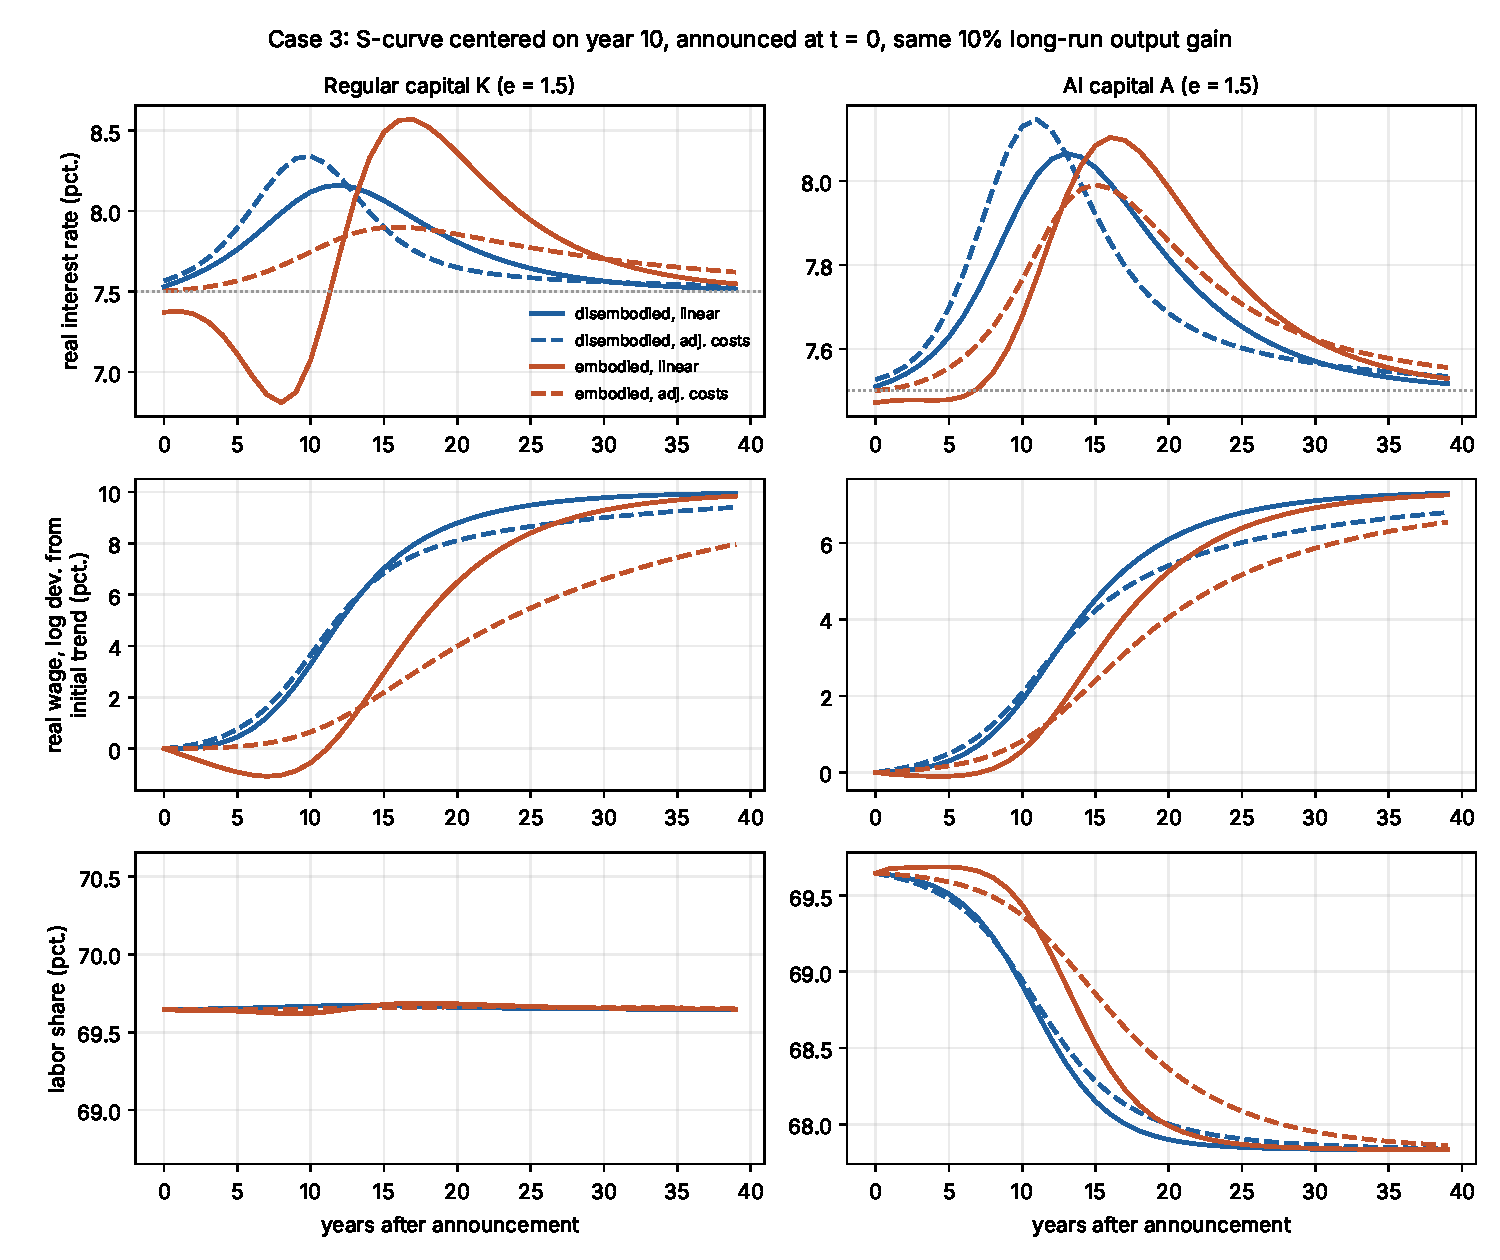
\includegraphics[width=\textwidth]{figures/fig_g_case3.pdf}
\caption{Case 3: S-curve centered on year 10, known at $t=0$, same 10\% long-run output gain.}\label{fig:c3}
\end{figure}

\begin{table}[h]\centering\scriptsize
\caption{Case 3: anticipated S-curve. Columns as in Table~\ref{tab:c1}.}\label{tab:c3}
\begin{tabular}{llccccccc}\toprule
 & & shock & $r_1$ & peak $r$ & year & $\ln W$, $t{=}10$ & $\ln W$, long run & labor share\\
 & & & (pct.) & (pct.) & & (pct.) & (pct.) & long run (pct.)\\\midrule
$K$ disemb. & linear & 0.255 & 7.53 & 8.16 & 12 & 3.3 & 10.0 & 69.6\\
$K$ disemb. & adj. costs & 0.255 & 7.57 & 8.34 & 10 & 3.7 & 10.0 & 69.6\\
$K$ emb. & linear & 0.255 & 7.37 & 8.57 & 17 & -0.6 & 10.0 & 69.6\\
$K$ emb. & adj. costs & 0.255 & 7.50 & 7.90 & 16 & 0.6 & 10.0 & 69.6\\
\midrule
AI disemb. & linear & 1.223 & 7.51 & 8.07 & 13 & 1.9 & 7.4 & 67.8\\
AI disemb. & adj. costs & 1.223 & 7.53 & 8.15 & 11 & 2.1 & 7.4 & 67.8\\
AI emb. & linear & 1.223 & 7.47 & 8.10 & 16 & 0.6 & 7.4 & 67.8\\
AI emb. & adj. costs & 1.223 & 7.50 & 7.99 & 15 & 0.8 & 7.4 & 67.8\\
\bottomrule\end{tabular}

\end{table}

\begin{enumerate}
\item \emph{Disembodied progress} raises $r$ gradually ahead of arrival. It peaks at 8.2--8.3
percent for regular capital and 8.1--8.15 percent for AI, around years 10--13. The wage
rises with the S-curve.
\item \emph{Embodied regular-capital progress with linear accumulation} produces a
two-phase response. Before the innovation arrives, firms let capital run down while
they wait for cheaper capital. The real rate \emph{falls} to about 6.8 percent around
year 8 and the wage dips by about 1 percent. Then an investment boom pushes $r$ to 8.6
percent in year 17. With adjustment costs, investment is spread out and $r$ rises
smoothly to 7.9 percent.
\item \emph{Embodied AI progress} shows the same pattern in muted form, with a small dip
before arrival and a peak of 8.0--8.1 percent around years 15--16.
\item \emph{AI versus regular capital.} For the same output gain, AI progress produces
similar or slightly smaller interest-rate peaks. It produces smaller wage gains (7.4 vs 10
percent) and a 1.8-point fall in the labor share that tracks the S-curve.
\end{enumerate}

\section{Summary}

\begin{itemize}
\item \emph{Wages.} For the same output gain, AI progress raises the wage by a fraction
$1/[1+(1-a)(\e-1)]$ of the output gain, and regular-capital progress raises it
one-for-one. The difference shows up as a lower labor share.
\item \emph{Interest rates after jumps and announcements.} Embodied progress, whether in
AI or regular capital, requires an investment boom and raises $r$ more on impact than
disembodied progress. Adjustment costs damp both responses.
\item \emph{Ongoing or anticipated embodied progress} can lower $r$ at first, because firms
wait for cheaper capital. The effect is strong with linear accumulation and largely
absent with adjustment costs. It is weaker for AI than for regular capital as long as
AI is a small share of capital.
\item \emph{Faster growth} raises $r$ one-for-one in the long run for every kind of
progress. With AI a substitute, permanently faster AI progress has no steady state.
The AI share and the interest rate keep rising.
\end{itemize}

\appendix
\section{Verification}
\texttt{growth\_cases.py} solves every experiment. It checks that the closed-form
balanced growth path satisfies the equilibrium conditions, that long-run output gains
match the target, and that the simulated growth rate converges to the closed form
in case 2.

\begin{table}[h]\centering\tiny
\begin{tabular}{lc}\toprule Check & max abs. error\\\midrule
e=1.5 adj=False: closed-form BGP satisfies equilibrium & 1.3e-15\\
e=1.5 adj=True: closed-form BGP satisfies equilibrium & 1.3e-15\\
e=1.0 adj=False: closed-form BGP satisfies equilibrium & 7.8e-16\\
e=1.0 adj=True: closed-form BGP satisfies equilibrium & 7.8e-16\\
level e=1.5 K dis lin: Newton residual & 1.1e-12\\
level e=1.5 K dis lin: long-run ln Y gain vs target & 3.0e-12\\
level e=1.5 K dis AC: Newton residual & 2.7e-12\\
level e=1.5 K dis AC: long-run ln Y gain vs target & 3.4e-08\\
level e=1.5 K emb lin: Newton residual & 4.9e-15\\
level e=1.5 K emb lin: long-run ln Y gain vs target & 1.3e-15\\
level e=1.5 K emb AC: Newton residual & 8.5e-13\\
level e=1.5 K emb AC: long-run ln Y gain vs target & 1.1e-07\\
level e=1.5 A dis lin: Newton residual & 2.3e-14\\
level e=1.5 A dis lin: long-run ln Y gain vs target & 5.4e-15\\
level e=1.5 A dis AC: Newton residual & 3.0e-15\\
level e=1.5 A dis AC: long-run ln Y gain vs target & 3.5e-08\\
level e=1.5 A emb lin: Newton residual & 2.2e-15\\
level e=1.5 A emb lin: long-run ln Y gain vs target & 1.3e-15\\
level e=1.5 A emb AC: Newton residual & 3.8e-13\\
level e=1.5 A emb AC: long-run ln Y gain vs target & 4.5e-08\\
growth e=1.5 K dis lin: Newton residual & 1.0e-14\\
growth e=1.5 K dis lin: growth at T vs closed form & 2.2e-16\\
growth e=1.5 K dis AC: Newton residual & 1.4e-12\\
growth e=1.5 K dis AC: growth at T vs closed form & 8.7e-11\\
growth e=1.5 K emb lin: Newton residual & 2.3e-15\\
growth e=1.5 K emb lin: growth at T vs closed form & 0.0e+00\\
growth e=1.5 K emb AC: Newton residual & 3.6e-14\\
growth e=1.5 K emb AC: growth at T vs closed form & 1.5e-10\\
growth e=1.0 K dis lin: Newton residual & 1.0e-14\\
growth e=1.0 K dis lin: growth at T vs closed form & 4.4e-16\\
growth e=1.0 K dis AC: Newton residual & 1.4e-12\\
growth e=1.0 K dis AC: growth at T vs closed form & 8.6e-11\\
growth e=1.0 K emb lin: Newton residual & 1.1e-15\\
growth e=1.0 K emb lin: growth at T vs closed form & 2.2e-16\\
growth e=1.0 K emb AC: Newton residual & 3.7e-14\\
growth e=1.0 K emb AC: growth at T vs closed form & 1.5e-10\\
growth e=1.0 A dis lin: Newton residual & 1.0e-14\\
growth e=1.0 A dis lin: growth at T vs closed form & 2.2e-16\\
growth e=1.0 A dis AC: Newton residual & 1.4e-12\\
growth e=1.0 A dis AC: growth at T vs closed form & 8.6e-11\\
growth e=1.0 A emb lin: Newton residual & 1.2e-11\\
growth e=1.0 A emb lin: growth at T vs closed form & 1.1e-15\\
growth e=1.0 A emb AC: Newton residual & 1.1e-13\\
growth e=1.0 A emb AC: growth at T vs closed form & 1.2e-10\\
scurve e=1.5 K dis lin: Newton residual & 9.4e-13\\
scurve e=1.5 K dis lin: long-run ln Y gain vs target & 2.5e-12\\
scurve e=1.5 K dis AC: Newton residual & 3.9e-12\\
scurve e=1.5 K dis AC: long-run ln Y gain vs target & 6.3e-08\\
scurve e=1.5 K emb lin: Newton residual & 4.1e-15\\
scurve e=1.5 K emb lin: long-run ln Y gain vs target & 9.3e-16\\
scurve e=1.5 K emb AC: Newton residual & 2.9e-13\\
scurve e=1.5 K emb AC: long-run ln Y gain vs target & 2.1e-07\\
scurve e=1.5 A dis lin: Newton residual & 1.9e-11\\
scurve e=1.5 A dis lin: long-run ln Y gain vs target & 8.8e-12\\
scurve e=1.5 A dis AC: Newton residual & 3.4e-11\\
scurve e=1.5 A dis AC: long-run ln Y gain vs target & 6.2e-08\\
scurve e=1.5 A emb lin: Newton residual & 1.8e-15\\
scurve e=1.5 A emb lin: long-run ln Y gain vs target & 6.9e-17\\
scurve e=1.5 A emb AC: Newton residual & 2.1e-15\\
scurve e=1.5 A emb AC: long-run ln Y gain vs target & 8.6e-08\\
\bottomrule\end{tabular}

\end{table}

\begin{thebibliography}{9}
\bibitem[Kiley(2000)]{kiley2000}
Kiley, M.~T. (2000). ``Stock Prices and Fundamentals in a Production Economy.''
FEDS Working Paper 2000-05, Federal Reserve Board.
\bibitem[Kiley(2004)]{kiley2004}
Kiley, M.~T. (2004). ``Stock Prices and Fundamentals: A Macroeconomic Perspective.''
\emph{Journal of Business} 77(4): 909--936.
\end{thebibliography}
\end{document}
